\documentclass[crop, border = 1bp]{standalone}

\usepackage{tikz}
\usetikzlibrary{positioning}

\begin{document}
\thispagestyle{empty}
%\begin{center}
%\makebox[\textwidth]{
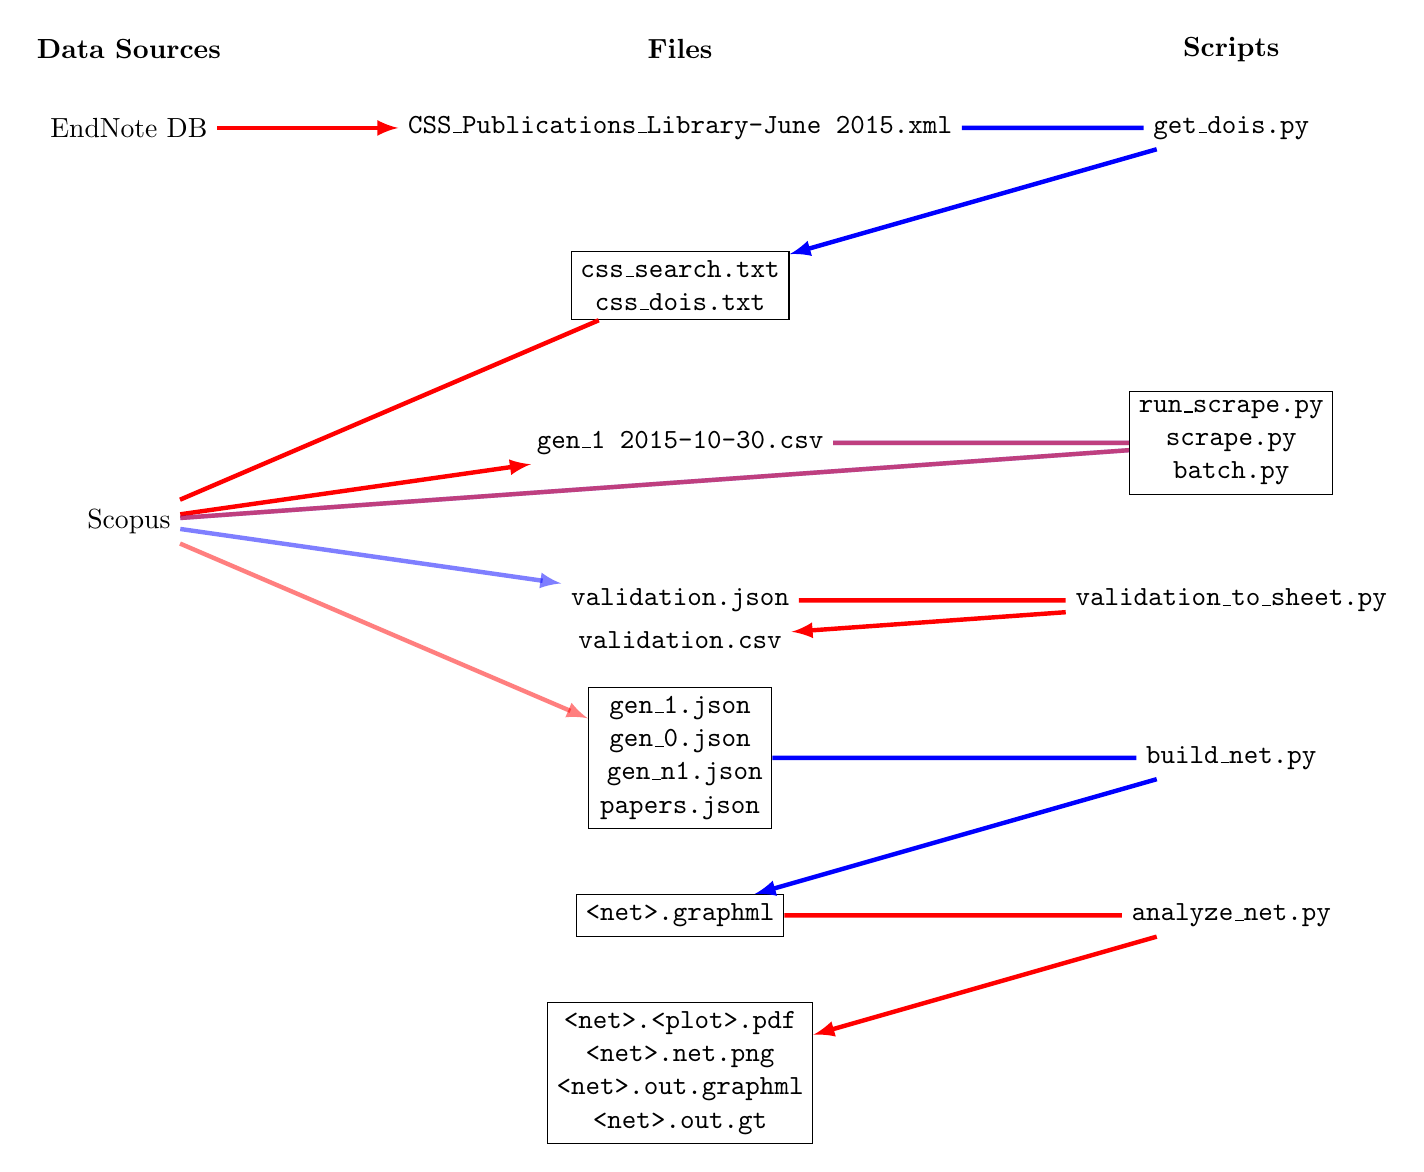
\begin{tikzpicture}[node distance = 2 and 7, on grid]
	%\draw[help lines] (0,0) grid (15, -21);
	\node (sourceshead) at (0,0) {\textbf{Data Sources}};
	\node (fileshead) [right = of sourceshead] {\textbf{Files}};
	\node (scriptshead) [right = of fileshead] {\textbf{Scripts}};
	
	\node (a) [below = 1 of sourceshead] {EndNote DB};
	\node (b) [right = of a] {\texttt{CSS\_Publications\_Library-June 2015.xml}};
	\node (c) [right = of b] {\texttt{get\_dois.py}};
	
	\node (d) [below left = of c, align = center, rectangle, draw] 
		{\texttt{css\_search.txt}\\
		 \texttt{css\_dois.txt}};
	
	\node (e) [below left = 3 and 7 of d] {Scopus};
	
	\node (f) [below = of d] {\texttt{gen\_1 2015-10-30.csv}};
	
	\node (g) [right = of f, align = center, rectangle, draw]
		{\texttt{run\_scrape.py}\\
		\texttt{scrape.py}\\
		\texttt{batch.py}};
	
	\node (h) [below = of f] {\texttt{validation.json}};
	
	\node (i) [below = of h, align = center, rectangle, draw] 
		{\texttt{gen\_1.json}\\
		\texttt{gen\_0.json}\\\
		\texttt{gen\_n1.json}\\
		\texttt{papers.json}};
		
	\node (j) [right = of h] {\texttt{validation\_to\_sheet.py}};
	\node (k) [below = .5 of h] {\texttt{validation.csv}};
	
	\node (l) [right = of i] {\texttt{build\_net.py}};
	\node (m) [below left = of l, align = center, rectangle, draw] 
		{\texttt{<net>.graphml}};
	
	\node (n) [right = of m] {\texttt{analyze\_net.py}};
	\node (o) [below left = of n, align = center, rectangle, draw]
		{\texttt{<net>.<plot>.pdf}\\
		\texttt{<net>.net.png}\\
		\texttt{<net>.out.graphml}\\
		\texttt{<net>.out.gt}};
	
	\begin{scope}[-latex, ultra thick]
		\draw[red] (a) -- (b);	
		\draw[blue] (b) -- (c) -- (d);
		\draw[red] (d) -- (e) -- (f);
		\draw[blue, opacity = .5] (f) -- (g) -- (e) -- (h);
		\draw[red, opacity = .5] (f) -- (g) -- (e) -- (i);
		\draw[red] (h) -- (j) -- (k);
		\draw[blue] (i) -- (l) -- (m);
		\draw[red] (m) -- (n) -- (o);
	\end{scope}
\end{tikzpicture}
%}
%\end{center}
\end{document}